\documentclass[preprint,12pt,authoryear]{elsarticle}

\usepackage{hyperref}
\usepackage{natbib}
\usepackage{graphicx}
\usepackage{ifthen}
\usepackage{tabularx}
\usepackage{lineno}
\linenumbers*[1]

% add references to research questions in margin
\newcommand{\mrq}[2][]{}
\newcommand{\rrq}[3][]{}
\newboolean{ispaper}
\setboolean{ispaper}{true}

\def\appendixname{}

\journal{Coastal Engineering}

\begin{document}

\begin{frontmatter}

  \title{Aeolian Sediment Supply at a Mega Nourishment}

  \author[tudelft,deltares]{Bas Hoonhout\corref{ca}}
  \ead{b.m.hoonhout@tudelft.nl}
  \ead{bas.hoonhout@deltares.nl}
  \cortext[ca]{Corresponding author}

  \author[tudelft]{Sierd de Vries}

  \address[tudelft]{Delft University of Technology, Faculty of Civil
    Engineering and Geosciences, Department of Hydraulic Engineering,
    Stevinweg 1, 2628CN Delft, The Netherlands.}

  \address[deltares]{Deltares, Department of Hydraulic Engineering,
    Boussinesqweg 1, 2629HV Delft, The Netherlands.}

  \begin{abstract}
    Mega nourishments are intended to enhance growth and resilience of
    coastal dunes on medium to long time scales by stimulation of
    natural sediment transport processes. The growth and resilience of
    coastal dunes largely depends on the presence of a continuous
    supply of aeolian sediment. A recent example of a mega nourishment
    is the 21 $\mathrm{Mm^3}$ mega nourishment known as the Sand
    Motor. The Sand Motor is intended to nourish the entire Holland
    coast over a period of two decades. Four years of bi-monthly
    topographic measurements of the Sand Motor domain provide an
    opportunity to analyze spatiotemporal variations in aeolian
    sediment supply using an aeolian sediment budget analysis. It
    appears that more than 58\% of all aeolian sediment deposits
    originate from the low-lying beaches that are regularly reworked
    by waves. Aeolian sediment supply from higher beaches diminished
    after half a year after construction of the Sand Motor, likely due
    to the formation of deflation lag deposits that constitute a beach
    armor layer. The compartmentalization of the Sand Motor in armored
    and unarmored surfaces suggests that the construction height is an
    important design criterion that influences the lifetime and region
    of influence for any mega nourishment.
  \end{abstract}

  \begin{keyword}
    aeolian sediment transport; aeolian sediment supply; beach
    armoring; sediment budgets; mega nourishment; Sand Motor
  \end{keyword}

\end{frontmatter}

\section{Introduction}

% context: intro nature-based flood defenses
Aeolian sediment supply is a prerequisite to growth and resilience of
coastal dunes that function as a natural protection against flooding
from the sea. Expanding human activities in coastal areas and growing
uncertainties related to climate change, increase coastal
risks. Mitigation of these risks resulted in the engineering of entire
coastlines \citep{Donchyts2016}. Rigid solutions and local
nourishments are traditional solutions to a societal demand for
coastal safety \citep{Hamm2002}. With the increased confidence in our
ability to mitigate coastal risks, additional demands and functions
for coastal flood protections arose. Soft engineering solutions with
limited environmental and ecological impact \citep{Waterman2010,
  deVriend2015} gained preference over rigid solutions or local
nourishments. Recently, the exponent of soft engineering emerged as
mega nourishments \citep{Stive2013}.  Mega nourishments pursue the
idea of stimulating natural sediment transport processes with the aim
of increasing coastal safety. The idea is based on the assumption that
the incidental or concentrated interventions necessary for the
stimulation of nature are less intrusive than classic solutions to
coastal safety. Moreover, mega nourishments tend to accommodate
long-term monitoring and periodic adaptation and intervention that
increases flexibility with respect to planning and execution as well
as the occurrence of coastal hazards. The increased flexibility can
make mega nourishments also cost-effective \citep{vanSlobbe2013}.

% context: role of aeolian sediment supply in nature-based flood defenses
The effectiveness of a mega nourishment depends on the sediment
transport pathways from nourishment to dunes. A small fraction of the
sediment moved in the nearshore ultimately arrives in the dunes
\citep{Aagaard2004}. It is this small aeolian sediment supply that
provides us with the natural and persistent coastal safety that mega
nourishments aim for. In addition, this small aeolian sediment supply
gives coastal dune systems the natural resilience to storm impacts and
the conditions for survival of persistent dune vegetation that
strengthens the dunes, like marram grass \citep{Borsje2011}. It is
also this small aeolian sediment supply that is least understood.

% what has been done?
Mega nourishments affect aeolian sediment supply to coastal dunes in
various ways. First, sand used for nourishment is typically obtained
from offshore borrowing pits and differs from the original beach sand
in terms of size and composition, affecting the erodibility of the
beach \citep{VanDerWal1998, VanDerWal2000}. Second, aeolian sediment
availability \citep[following the definition of][]{Kocurek1999} at
beach nourishments that are constructed above storm surge level can be
significantly reduced by deflation lag deposits
\citep{Jackson2010}. The absence of regular flooding and
wave-reworking allows lag deposits to develop a beach armor layer,
resulting in compartmentalization of the nourishment in armored and
unarmored surfaces. \citet{McKennaNeuman2012} illustrated how
deflation lag deposits increase the shear velocity threshold
significantly and reduce aeolian sediment availability and
subsequently supply from the higher supratidal beach. Deflation lag
deposits can therefore cause intertidal and low-lying supratidal
beaches to gain importance over the high and dry beach as source of
aeolian sediment. Third, the placement of a nourishment is known to
affect nearshore processes \citep{Grunnet2005, Ojeda2008,
  deSchipper2013}.  Synchronization between aeolian and nearshore
processes, like onshore bar migration and welding, is reported to
stimulate aeolian sediment supply to coastal dunes \citep{Houser2009,
  Anthony2013}. The importance of low-lying beaches as source of
aeolian sediment might therefore also be affected by changing bar
dynamics.
% , resulting in a complex morphological interplay between nourishment
% and aeolian sediment supply.

%\citep{Jackson1999, DavidsonArnott2005,
%  DavidsonArnott2008, Bauer2009}. Fetch is important as a certain
%distance is required for the development of a saturated saltation
%cascade. Because the saltation cascade develops slower when sediment
%is scarce, the critical fetch is inversely proportional to the
%sediment availability \citep{DelgadoFernandez2010}. In coastal
%environments the available fetch is often limited and depends on, for
%example, the wind direction. If the available fetch is shorter than
%the critical fetch, the wind transport capacity is not a reliable
%indicator for the actual sediment flux \citep{Bauer2002}
%
%

%Jackson2010
%measurements, models
%small nourishments
%short time scales
%nourishment strategies
%quantification
%dynamic

% what do we need?
\citet{Jackson2011} emphasized the necessity for the quantification of
the effect of large scale beach nourishment designs on aeolian
sediment supply. Quantitative predictions of aeolian sediment
availability and supply in coastal environments has proven to be
challenging \citep{Sherman1998, Sherman2012}. Limitations in aeolian
sediment availability are often identified as reason for the
discrepancy between measured and predicted sediment transport rates
\citep{DelgadoFernandez2012, deVries2014b, Lynch2016}.

Mega nourishments inherently cause spatiotemporal variations in
aeolian sediment availability. The spatial variations are caused by
compartmentalization of the beach. The temporal variations are induced
by adaptation of the large coastal disturbance to the wave and wind
climate, resulting in changing in beach width, slope and composition
\citep{deSchipper2016}. Consequently, quantification of aeolian
sediment availability and supply from mega nourishments requires
differentiation in space and time.

% what did we do?
This paper presents an aeolian sediment budget analysis of the 21
$\mathrm{Mm^3}$ Sand Motor mega nourishment based on four years of
bi-monthly topographic surveys. The sediment budget analysis
quantifies the net aeolian sediment supply to the dunes, dune lake and
lagoon accommodated by the Sand Motor. The Sand Motor constitutes
distinct areas that are either influenced by marine processes, by
aeolian processes or by a combination of both. Therefore, the
influence of marine and aeolian processes on aeolian sediment supply
can be separated and spatiotemporal variations in aeolian sediment
availability can be identified with reasonable accuracy. The observed
compartmentalization of the Sand Motor is discussed in relation to
limitations in aeolian sediment availability, as well as the design of
mega nourishments like the Sand Motor as solution to coastal safety.

%evaluation of mega-nourishment sand motor wrt ordinary nourishment as natural supplier of aeolian sediment
%role of dune lake and lagoon
%long-term aeolian sediment budget analysis
%identifies source and deposition area
%quantifies aeolian sediment supply
%lessons learned for mega nourishments


%% context
%The wind transport capacity is a poor indicator for the actual aeolian
%sediment transport rate in coastal environments \citep{Sherman1998,
%  Sherman2012}. Limitations in sediment availability \citep[following
%the definition of][]{Kocurek1999} are often identified as reason for
%the discrepancy between measured sediment transport rates and the wind
%transport capacity \citep[e.g.][]{Houser2009, DelgadoFernandez2012,
%  deVries2014b}. The sediment availability can be limited by a variety
%of bed surface properties; for example soil moisture is known to limit
%the sediment availability significantly \citep{Wiggs2004, Edwards2009,
%  Namikas2010}. An example of an availability-limited coastal system
%is the Sand Motor mega nourishment \citep[or Sand
%Engine;][]{Stive2013} where aeolian sediment transport rates only
%reach to about 25\% of the estimated wind transport
%capacity. Moreover, the Sand Motor accommodates a large spatial
%variation in bed surface properties and therefore provides a unique
%opportunity to investigate the influence of bed surface properties on
%coastal aeolian sediment transport and dune growth.
%
%% what has been done?
%Although consensus may exist that limitations in sediment availability
%are important for coastal aeolian sediment transport, it is still
%being debated how sediment availability influences aeolian sediment
%transport and how this influence can be measured best. Measurements on
%the influence of bed surface properties on the sediment availability
%date from the 1930's with the pioneering work of \citet{Bagnold1937b}
%and gained significant interest from the 1960's onward
%\citep[e.g.][]{Belly1964, Howard1977, Dyer1986, Gillette1989}. Studies
%on specific bed surface properties are typically performed in a wind
%tunnel and define an adapted threshold velocity that relates the
%theoretical wind transport capacity to a measured sediment transport
%capacity. In the new millennium an increasing number of field
%measurements is dedicated to the influence of sediment availability on
%aeolian sediment transport in coastal environments. Field measurements
%are typically performed in an attempt to find a distance at which
%saturated transport is reached: the critical fetch \citep{Jackson1999,
%  DavidsonArnott2005, DavidsonArnott2008, Bauer2009}. Fetch is
%important as a certain distance is required for the development of a
%saturated saltation cascade. Because the saltation cascade develops
%slower when sediment is scarce, the critical fetch is inversely
%proportional to the sediment availability
%\citep{DelgadoFernandez2010}. In coastal environments the available
%fetch is often limited and depends on, for example, the wind
%direction. If the available fetch is shorter than the critical fetch,
%the wind transport capacity is not a reliable indicator for the actual
%sediment flux \citep{Bauer2002}. As the critical fetch is relatively
%easy to measure, the critical fetch concept provides a convenient
%framework for field measurements. However, measurements on the
%critical fetch assume that, in case of sufficient fetch, saturated
%transport will be reached. In a truly availability-limited system this
%assumption is not necessarily valid: an increasing wind transport
%capacity or fetch will not lead to an increase in transport if no
%additional sediment is available. The subtle difference is especially
%important for nourished coasts for which sand is extracted from
%offshore borrowing pits.\mrq[ls]{1.6} Such coasts tend to contain many
%shells, shell fragments and other roughness elements that cause a
%significant limitation and spatiotemporal variability in sediment
%availability \citep{VanDerWal1998, VanDerWal2000,
%  McKennaNeuman2012}. When sediment availability is severely limited
%and is varying spatially, the critical fetch may become very large,
%highly variable or even undefined, which makes the definition and
%interpretation of the critical fetch impractical
%\citep{Lynch2016}. Recently, \citet{deVries2014a} proposed an
%alternative conceptual approach that is based on an explicit
%definition of sediment availability. This approach makes the
%assumption that saturated sediment transport is reached, given
%sufficient fetch, unnecessary. % \citet{Hoonhout2016} continue on this
%% approach by defining the sediment availability in terms of
%% (measurable) bed surface properties, like grain size, roughness
%% density and moisture content.
%
%% what do we need?
%% The explicit relation between bed surface properties and sediment
%% availability proposed by \citet{Hoonhout2016} provides a framework in
%% which the influence of arbitrary configurations of bed surface
%% properties on aeolian sediment availability and transport can be
%% described.
%Aeolian sediment availability or supply can be quantified explicitly
%in the field by a sediment budget analysis. A sediment budget analysis
%compares changes in sediment volumes between different pre-defined
%control areas. The control areas are defined such that homogeneous bed
%surface properties and sediment availability can be assumed within
%each control area. The analysis therefore provides insight in the
%relation between bed surface properties, sediment availability and
%supply. A major advantage of this approach is that regular topographic
%measurements can be used to directly measure the influence of sediment
%availability on aeolian sediment transport, even in complex coastal
%environments.
%
%% what did we do?
%This paper presents an extensive aeolian sediment budget analysis of
%the Sand Motor based on four years of bi-monthly topographic surveys
%\citep{deSchipper2016}. The sediment budget analysis localizes and
%quantifies spatial variations in sediment supply in the Sand Motor
%region. Despite the uniqueness of the Sand Motor, the properties and
%processes limiting aeolian sediment transport and dune growth are
%common and relevant for (nourished) beaches worldwide.

\section{Field Site}
\label{sec:fieldsite}

The Sand Motor (or Sand Engine) is an artificial 21 $\mathrm{Mm^3}$
sandy peninsula protruding into the North Sea off the Delfland coast
in The Netherlands \citep[Figure \ref{fig:fieldsite},][]{Stive2013}.
The Sand Motor is an example of a mega nourishment and is intended to
nourish the Holland coast for a period of two decades, while
stimulating both biodiversity and recreation.

\begin{figure}
  \centering
  \includegraphics[width=\columnwidth]{../Figures/location_and_evolution}
  \caption{Location, orientation, appearance and evolution of the Sand
    Motor between construction in 2011 and 2015. The box indicates the
    measurement domain used in the remainder of this paper. A 100 x
    100 m grid aligned with the measurement domain is plotted in gray
    as reference.}
  \label{fig:fieldsite}
\end{figure}

The Sand Motor was constructed in 2011 and its bulged shoreline
initially extended about 1 km seaward and stretched over approximately
2 km along the original coastline. The original coast was
characterized by an alongshore uniform profile with a vegetated dune
with an average height of 13 m and a linear beach with a 1:40
slope. The dune foot is located at a height of approximately 5 m+MSL.

Due to natural sediment dynamics the Sand Motor distributes about 1
$\mathrm{Mm^3}$ of sand per year to the adjacent coasts (Figure
\ref{fig:fieldsite}). The majority of this sand volume is transported
by tides and waves. However, the Sand Motor is constructed up to 5
m+MSL and locally up to 7 m+MSL, which is in either case well above
the maximum surge level of 3 m+MSL (Figure
\ref{fig:windwaves}c). Therefore, the majority of the Sand Motor area
is uniquely shaped by wind.

The Sand Motor comprises both a dune lake and a lagoon that act as
large traps for aeolian sediment (Figure \ref{fig:fieldsite}). The
lagoon is affected by tidal forcing, although the tidal amplitude
quickly diminished over time as the entry channel elongated. The tidal
range of about 2 m that is present at the Sand Motor periphery (Figure
\ref{fig:windwaves}c), is nowadays damped to less than 20 cm inside
the lagoon \citep{deVries2015}. Consequently, the tidal currents at
the closed end of the lagoon, where most aeolian sediment is trapped,
are negligible.

Sand used for construction of the Sand Motor is obtained from an
offshore borrowing pit in the North Sea. The sand is predominantly
Holocene sand with a significant amount of fines. The median grain
size is slightly coarser than found originally along the Delfland
coast. Apart from sand fractions, the sediment contains a large amount
of shells, shell fractions, some pebbles and cobbles and an occasional
fraction of a mammoth bone.

%\begin{figure}
%  \centering
%  \includegraphics[width=\columnwidth]{../Figures/grainsize}
%  \caption{Evolution of the grain size distribution at the dry beach
%    since 2010, prior to construction of the Sand Motor
%    \citep{ImaresSamples}. Left panel: time series of median grain
%    size. Right panel: grain size distributions.}
%  \label{fig:grainsize}
%\end{figure}

The dominant wind direction at the Sand Motor is south to southwest
(Figure \ref{fig:windwaves}a). However, during storm conditions the
wind direction tends to be southwest to northwest. During extreme
storm conditions the wind direction tends to be
northwest. Northwesterly storms are typically accompanied by
significant surges as the fetch is virtually unbounded to the
northwest, while surges from the southwest are limited due to the
presence of the narrowing of the North Sea at the Strait of Dover
(Figure \ref{fig:fieldsite}, inset).

\begin{figure}
  \centering
  \includegraphics[width=\columnwidth]{../Figures/boundaryconditions}
  \caption{Wind and hydrodynamic time series from 2011 to 2015. Hourly
    averaged wind speeds and directions are obtained from the KNMI
    meteorological station in Hoek van Holland (upper
    panels). Offshore still water levels, wave heights and wave
    periods are obtained from the Europlatform (lower panels). Runup
    levels are estimated following \citet{Stockdon2006}.}
  \label{fig:windwaves}
\end{figure}

%The 21 $\mathrm{Mm^3}$ Sand Motor mega nourishment provides a unique
%opportunity to investigate the relation between bed surface
%properties, spatiotemporal variations in sediment availability, supply
%and aeolian sediment transport. At the Sand Motor, limitations in
%fetch are negligible as fetches can exceed 1.0 km depending on the
%location and wind direction. In addition, the Sand Motor accommodates
%a large spatiotemporal variability in bed surface properties:
%expanding moist intertidal beaches, pronounced intertidal bar dynamics
%and vast dry areas that are severely armored by the emergence of
%shells, shell fragments and other roughness elements that are
%contained by the sand from offshore borrowing pits. 

\section{Methodology}

Spatiotemporal variations in aeolian sediment supply in the Sand Motor
domain are identified using an aeolian sediment budget analysis. A
sediment budget analysis can be performed if frequent topographic
measurements are available \citep{DavidsonArnott1990} and sediment
exchange over the border of the measurement domain is limited. In a
sediment budget analysis the morphological change in predetermined
areas are converted to volumetric changes (budgets) that are compared
in a sediment volume balance.

A sediment budget analysis is particularly suitable for coastal sites
with a complex and dynamic topography, like the Sand Motor. The use of
(dense) topographic measurements ensures that any local variations in
the topography are included. Moreover, no assumptions on the local
representativeness of the measurements are needed. The methodology is
applicable to a wide range of spatial or temporal scales, allowing a
multi-annual analysis of aeolian sediment supply in the Sand Motor
domain.

In the Sand Motor domain it is possible to separate the marine and
aeolian influence on erosion and deposition of sediment directly from
a sediment budget analysis. The high construction height of the Sand
Motor and the absence of regular storm surges in the first four years
after construction make that distinct areas exist that are either
influenced by marine or aeolian processes. The sediment budgets are
determined along the borders of these marine and aeolian zones.

%An aeolian sediment budget analysis has several advantages with
%respect to traditional measurements techniques, like sediment traps or
%saltation measurements, for the purpose of quantification of
%multi-annual aeolian sediment supply. Multi-annual deployment of
%sediment traps or saltation measurements in the Sand Motor domain is
%complicated by:
%
%
%\begin{enumerate}
%\item A complex, non-uniform topography that would require a large
%  number of measurement locations to account for the spatial variation
%  in aeolian sediment transport;
%\item A dynamic topography that would require constant relocation and
%  maintenance of instrumentation to prevent blocking, clogging or loss
%  of the instrumentation;
%\item The public accessibility of the area that would require constant
%  monitoring of instrumentation to prevent the measurements being
%  compromised;
%\item The necessity to translate trapped sediment volumes and/or
%  saltation rates to large scale sediment volumes, which would require
%  more extensive assumptions on the local representativeness of the
%  data than required in a sediment budget analysis.
%\end{enumerate}

\subsection{Topographic measurements}

32 topographic measurements of the Sand Motor domain obtained over a
period of four years are used to determine the overall sediment budget
of the Sand Motor domain \citep{deSchipper2016}. The measurement area
covers 1.4 km cross-shore and 4 km alongshore (Figure
\ref{fig:fieldsite}). The nearshore bathymetry is surveyed using a
jetski equipped with an echo sounder and RTK-GPS receiver. The
topography of the Sand Motor from the waterline up to the dune foot is
surveyed using an all-terrain vehicle (ATV) that is also equipped with
a RTK-GPS receiver. Inundated areas that are too shallow for the
jetski, like the tidal channel and the dune lake, are surveyed using a
manually pushed RTK-GPS wheel. The survey is performed along
cross-shore transects that are 20 m apart. The resulting trajectories
are interpolated to a regular 10 m x 10 m grid for the sediment budget
analysis. Surveys that show a morphological rate of change that is
more than two standard deviations from the average are considered
outliers. The measurements of September 4, 2011 and June 21, 2012 are
discarded as outliers.

The topography in the dune area, which is not included in the RTK-GPS
surveys, is monitored by airborne lidar. Half-yearly measurements from
the southern Holland coast (Delfland coast) are available since 2011,
prior to the construction of the Sand Motor. The lidar measurements
have a spatial resolution of 2 m or 5 m. The measurements are
corrected for the presence of vegetation and artificial objects, like
beach pavilions, and interpolated to the same 10 m x 10 m grid and the
same moments in time as the RTK-GPS measurements.

\subsection{Zonation}
\label{sec:zonation}

\begin{figure}
  \centering
  \includegraphics[width=\columnwidth]{../Figures/decomposition}
  \caption{Zonation of the Sand Motor domain into zones with net
    aeolian erosion and no marine influence, net aeolian deposition
    and no marine influence, mixed aeolian/marine influence and marine
    influence. Left panels: 2011. Right panels: 2015.}
  \label{fig:decomposition}
\end{figure}

The Sand Motor domain is divided into seven zones for the aeolian
sediment budget analysis (Table \ref{tab:decomposition} and Figure
\ref{fig:decomposition}). The zonation aims to separate areas with
marine influences from areas without marine influences, and separate
areas with net aeolian erosion from areas with net aeolian deposition.

\begin{table}[h!]
  \centering
  \caption{Zonation of the Sand Motor domain into seven zones with and
    without marine influence. See also Figure \ref{fig:decomposition}.}
  \label{tab:decomposition}
  \begin{tabularx}{\textwidth}{XX}
    \emph{without} marine influence  & \emph{with} marine influence \\
    \hline
    aeolian zone                     & mixed zone (north)           \\
    dunes                            & mixed zone (south)           \\
    dune lake                        & marine zone                  \\
    lagoon                           &                              \\
  \end{tabularx}
\end{table}

The zonation is based on the 0 m+MSL, 3 m+MSL and 5 m+MSL contour
lines that roughly correspond to mean sea level, the edge of the berm
or maximum runup level (Figure \ref{fig:windwaves}c) and the dune foot
respectively. The contours are determined such that the spatial
variance in the bed level change of the zones is minimized. The
minimization ensures that the optimal division between erosion and
deposition areas is found. Moreover, the 3 m+MSL and 5 m+MSL contour
lines have been relatively static since construction of the Sand
Motor.

To ensure a constant shape and size of the zones during the analysis,
the convex hull of all 3 m+MSL contour lines is used as zone boundary
for the lake and lagoon. Also for the dunes minimal variations over
time in zone shape and size are removed by using the most seaward
position of all contour lines. Consequently, only the aeolian zone and
mixed zones change in shape and size over time. The volumetric change
between two consecutive measurements is determined for these zones
within the smaller contour:

\begin{equation}
  \Delta V^n = \hat{A}_{\mathrm{c}} \cdot \left( \overline{z_{\mathrm{b}}}^n - \overline{z_{\mathrm{b}}}^{n-1} \right)
  \quad \mathrm{where} ~ \hat{A}_{\mathrm{c}} = \min \left( A_{\mathrm{c}}^n ~;~ A_{\mathrm{c}}^{n-1} \right)
\end{equation}

\noindent with $\Delta V^n$ the volume change, $A_{\mathrm{c}}^n$ the
surface area of the zone and $\overline{z_{\mathrm{b}}}^n$ the average
bed level in the zone, all in time interval $n$. The (cumulative) sum
over all time intervals of the volume changes in each zone is used in
the analysis. By using the smaller of two contours in a comparison, a
part of the larger contour is neglected:

\begin{equation}
  A^n_{\mathrm{c,neglected}} = \max \left( A_{\mathrm{c}}^n ~;~ A_{\mathrm{c}}^{n-1} \right) - \hat{A}_{\mathrm{c}}
\end{equation}

\noindent The neglected area of the zone with the largest change in
size, the aeolian zone, is on average 2\% and never larger than 8\%.

\subsection{Spatial variations in porosity}

The change in sediment volume is susceptible to changes in
porosity. In order to relate the changes in sediment volume to the
transport of sediment mass, variations in porosity need to be
accounted for. Porosity values in the Sand Motor domain are obtained
from core samples and used to account for the spatial variations in
porosity. The core samples have a diameter of 8 cm and depth of 10 cm
from the bed surface in an attempt to capture the porosity in the
aeolian active layer of the bed. Each sample is dried and submerged in
water to determine the porosity. For comparison, all presented
sediment volumes in this paper are converted to a hypothetical
porosity of 40\% according to:

\begin{equation}
  V_{\mathrm{40\%}} = V \cdot \frac{1 - p}{1 - 40\%}
\end{equation}

\noindent where $V$ [$\mathrm{m^3}$] is the measured sediment volume
and $p$ [-] the porosity.

\section{Results}

\begin{figure}
  \centering
  \includegraphics[width=\columnwidth]{../Figures/sedero}
  \caption{Yearly sedimentation and erosion above 0 m+MSL in the Sand
    Motor domain. Comparisons are made between the September surveys
    of each year.}
  \label{fig:sedero}
\end{figure}

The overall sediment budget of the Sand Motor domain is determined
given morphological change in the net aeolian erosion and net aeolian
deposition zones for the period between September 1, 2011 and
September 1, 2015 (Figure \ref{fig:sedero}).

\subsection{Morphological change and porosity}

The net morphological change within the 3 m+MSL contour can be
accredited entirely to aeolian sediment transport as this area is not
significantly affected by marine processes since the construction of
the Sand Motor. Also the net contribution of alongshore sediment
fluxes are assumed to be relatively small given that the beach width
($<$ 100 m) is small compared to the alongshore span of the
measurement domain (4 km). Within the 3 m+MSL contour sediment is
deposited in the dunes and eroded from the aeolian zone.

The morphological change in the dune lake and the closed end of the
lagoon is assumed to be driven predominantly by wind. Hydrodynamic
forcing and consequently marine deposits in these zones diminished
quickly over time, while significant amounts of fine aeolian deposits
are found along the southwestern to northwestern shores. \mrq[ls]{1.3}

The aeolian contribution to the morphological change in the mixed
zones cannot be determined directly due to the presence of both marine
and aeolian forces. However, by balancing the changes in sediment
volume in the net aeolian deposition zones with the changes in
sediment volume in the net aeolian erosion zones the aeolian sediment
supply from the mixed zones is estimated. \mrq[ls]{1.1}

18 porosity measurements from six zones (Table \ref{tab:porosity}) are
used to convert all measured sediment volumes to a hypothetical
porosity of 40\%.

\begin{table}
  \centering
  \caption{Measured porosity values in the Sand Motor domain. Each
    area is sampled at three different locations. The results per area are
    presented in ascending order. The last column presents the average
    porosity for each area that is used to convert the sediment volumes
    presented in this paper to a hypothetical porosity of 40\%.}
  \label{tab:porosity}
  \begin{tabular}{lrrrr}
    Area                     & \multicolumn{4}{c}{Porosity}      \\
                             & min.   &        & max.   & avg.   \\
    \hline 
    Aeolian zone             & 39.0\% & 39.4\% & 40.2\% & 39.5\% \\
    Mixed zone (north)       & 38.4\% & 39.8\% & 40.8\% & 39.7\% \\
    Mixed zone (south)       & 37.1\% & 38.4\% & 38.4\% & 38.0\% \\
    Dunes                    & 36.1\% & 36.3\% & 37.1\% & 36.5\% \\
    Dune lake                & 34.7\% & 34.9\% & 36.3\% & 35.3\% \\
    Lagoon                   & 46.3\% & 47.3\% & 49.0\% & 47.6\% \\
  \end{tabular}
\end{table}

\subsection{Aeolian sediment budgets}
\label{sec:budgets}

\begin{figure}
  \centering
  \includegraphics[width=\columnwidth]{../Figures/volumes_bars}
  \caption{Aeolian sediment budgets in the Sand Motor domain in the
    period between September 1, 2011 and September 1, 2015.}
  \label{fig:volumes_bars}
\end{figure}

The aeolian zone consistently provides less sediment than is deposited
in the dunes, dune lake and lagoon (Figure
\ref{fig:volumes_bars}). Over the four years since construction of the
Sand Motor the volume deficit accumulates to $\mathrm{21 \cdot 10^4}$
$\mathrm{m^3}$, which is 52\% of the total sediment accumulation of
$\mathrm{40 \cdot 10^4}$ $\mathrm{m^3}$. \mrq[ls]{1.2} The total wind
transport capacity (or cumulative theoretical sediment transport
volume) in this period is roughly estimated as
$\mathrm{110 \cdot 10^4}$ $\mathrm{m^3}$ (Appendix
\ref{apx:theoretical_transport}). As the actual sediment transport
rates appear to be only about 35\% of the wind transport capacity, the
Sand Motor can be classified as an availability-limited system.

Late January 2012, the surveys show a net volume deficit of zero,
while subsequent surveys show a more or less linear growth of the
volume deficit (Figure \ref{fig:netvolumechange}). Fitting a linear
trend reveals an average growth rate of $\mathrm{5.2 \cdot 10^4}$
$\mathrm{m^3/yr}$, which is 67\% of the total sediment accumulation
rate of $\mathrm{7.7 \cdot 10^4}$ $\mathrm{m^3/yr}$ ($\mathrm{R^2}$ =
0.96). The increase in growth rate of the volume deficit is likely
caused by a significant decrease of the sediment contribution from the
aeolian zone. The erosion from the aeolian zone in the first half year
after construction of the Sand Motor exceeds the total erosion in the
four years thereafter, while sediment continued to be accumulated in
the dunes, dune lake and lagoon. The surface area of the aeolian zone
decreased continuously (Figure \ref{fig:areas}).

\begin{figure}
 \centering
  \includegraphics[width=\columnwidth]{../Figures/netvolumechange}
  \caption{Cumulative change in sediment volume of all net aeolian
    erosion and net aeolian deposition zones and the volume
    deficit. For the linear fit the period prior to February 2012 is
    discarded (shaded).}
  \label{fig:netvolumechange}
\end{figure}

\begin{figure}
  \centering
  \includegraphics[width=\columnwidth]{../Figures/areas}
  \caption{Change in size of aeolian zone and mixed zones since
    construction of the Sand Motor in 2011.}
  \label{fig:areas}
\end{figure}

The diminishing of the aeolian sediment supply from the aeolian zone
is also reflected in the average bed level within the 3 m+MSL contour
of September 22, 2015 (Figure \ref{fig:heights}). The bed level within
this contour has been almost constant since the volume deficit started
to grow steadily from late January 2012. Only a few periods of
significant erosion can be distinguished that can be related to storm
events. Most notably, the event of December 5, 2013 with wind speeds
up to 34 m/s. That day $\mathrm{1.5 \cdot 10^4}$ $\mathrm{m^3}$ of
sediment was eroded from within the 3 m+MSL contour of September 22,
2015, which is 52\% of the total erosion that year. Although this
event is among the few events during which the runup levels exceeded
the 3 m+MSL level (Figure \ref{fig:windwaves}), the erosion can still
be accredited to wind as the 3 m+MSL contour of September 22, 2015 was
located about 100 m landward of the 3 m+MSL contour at the time of the
storm event. Therefore the bed level in the more recent contour was
not affected by the surge, which is confirmed by observations from a
local permanent camera station.% (Figure \ref{fig:argus}).

In general, the use of the 3 m+MSL contour as divide between the areas
with and without marine influence appears to be valid for almost the
entire four years after construction of the Sand Motor. Only four
events have been registered in which runup levels exceeded the 3 m+MSL
level (Figure \ref{fig:windwaves}). Observations from a local
permanent camera station indicate that only during the event of
December 5, 2013 the surface of the aeolian zone was significantly
affected by tides and waves. Pre- and post-storm topographic surveys
that are available for this event indicate that the marine erosion
from the flooded areas above the 3 m+MSL level was less than
$\mathrm{1 \cdot 10^4}$ $\mathrm{m^3}$.

%Additional visual observations of the Sand Motor surface indicate that
%a coarse beach armor layer developed over time that consists of coarse
%sand, shell fragments and shells.% (Figure \ref{fig:armoring}).

\begin{figure}
  \centering
  \includegraphics[width=\columnwidth]{../Figures/heights}
  \caption{Average height of the aeolian zone in the most recent
    contour.}
  \label{fig:heights}
\end{figure}

%\begin{figure}
%  \centering
%  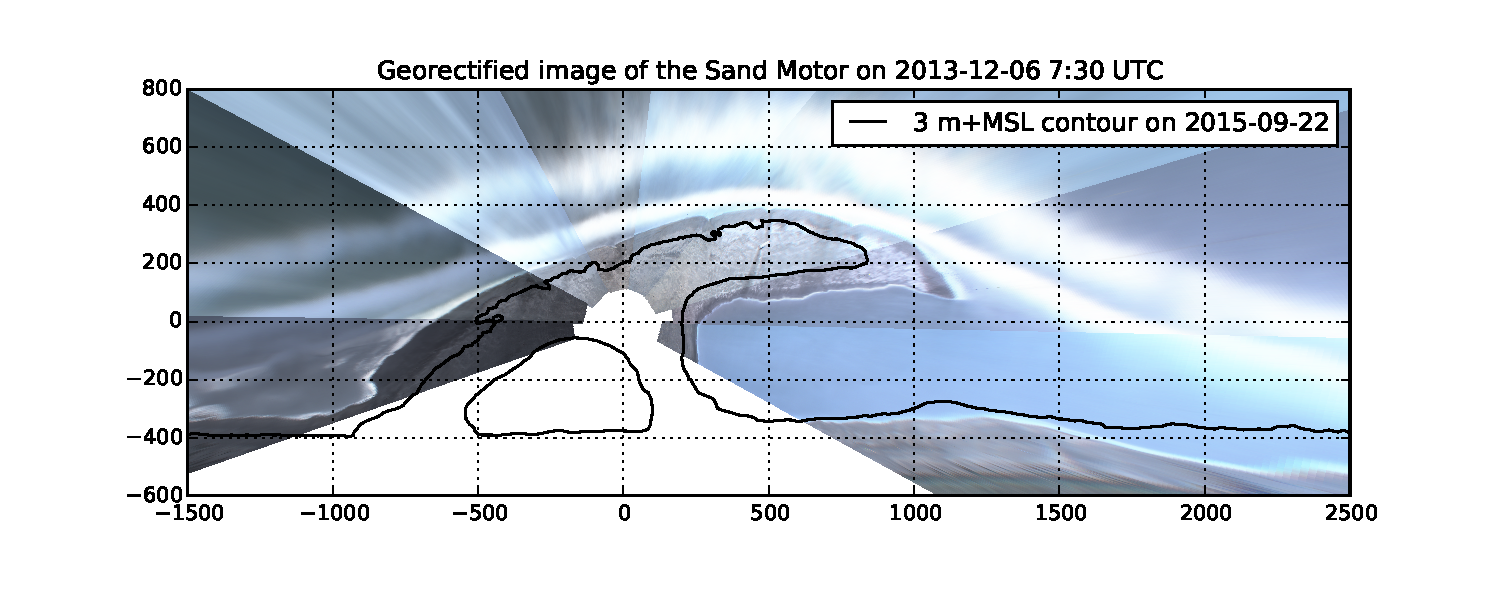
\includegraphics[width=\columnwidth]{../Figures/argus}
%  \caption{Image from the local permanent camera station at the Sand
%    Motor from December 6, 2013 with the 3 m+MSL contour of September
%    22, 2015. The image is georectified using the \textsc{Flamingo}
%    toolbox \citep{Hoonhout2015a}.}
%  \label{fig:argus}
%\end{figure}

%\begin{figure}
%  \centering
%  \includegraphics[width=\columnwidth]{../Figures/armoring_small}
%  \caption{Visual impression of armor layer at three locations in the
%    Sand Motor region: a) intertidal beach, no armoring b) lower dry
%    beach, minor armoring with shell fragments c) upper dry beach,
%    severe armoring with many shells and coarse sand. Covered surface
%    is approximately 40 cm x 40 cm in all cases.}
%  \label{fig:armoring}
%\end{figure}

\subsection{Alongshore variation}

The sediment deposits in the dunes show an alongshore
variation\mrq[ls]{2.4}. A depression in dune growth is observed in the
lee of the dune lake and lagoon (Figure
\ref{fig:adjacentcoasts}). South of the dune lake and in between the
dune lake and lagoon a passage for aeolian sediment transport is
present, which seems to result in a locally elevated dune growth. The
average dune growth of 14 $\mathrm{m^3/m/yr}$ in the Sand Motor domain
is low compared to the dune growth rate along the adjacent southern
(15 $\mathrm{m^3/m/yr}$) and northern (19 $\mathrm{m^3/m/yr}$) beach
stretches.  However, aeolian deposits in the dune lake and lagoon are
of the same order of magnitude resulting in a total average sediment
deposition of 27 $\mathrm{m^3/m/yr}$ in the Sand Motor domain, which
is on average 56\% higher than along the adjacent coasts.

\begin{figure}
 \centering
  \includegraphics[width=\columnwidth]{../Figures/adjacentcoasts}
  \caption{Comparison sediment accumulation rates in dunes
    (\textgreater 3 m+MSL) for Sand Motor domain and adjacent
    coasts. Airborne lidar measurements from January 2012 until
    January 2015 are used. Horizontal dashed lines indicate local
    averages. The box indicates the Sand Motor domain depicted in
    previous figures.}
  \label{fig:adjacentcoasts}
\end{figure}

\section{Discussion}

% southern intertidal beach is main supplier of aeolian sediment
The volume deficit between the net aeolian erosion and net aeolian
deposition zones can be accredited to the mixed zones that are
affected by both marine and aeolian processes. The mixed zones in the
Sand Motor domain are consequently estimated to provide 67\% of the
aeolian sediment in the Sand Motor domain. \mrq[ls]{1.4} The aeolian
sediment supply from the mixed zones is therefore significant, but
still small compared to the 98\% reported by \citet{Jackson2010}. The
importance of the mixed zone cannot be explained by the size of the
surface area as the mixed zones are initially smaller than the other
main sediment source: the aeolian zone (Figure \ref{fig:areas}). Only
from 2013 onward the surface area of the mixed zones exceed the area
of the aeolian zone. However, the increase in surface area of the
mixed zones is concentrated in the north where a low-lying spit
develops (Figure \ref{fig:sedero}). Given the dominant south to
southwesterly wind direction and their position with respect to the
lagoon that separates the spit from the dunes, it is unlikely that
these intertidal beaches, provide a significant amount of sediment to
dunes, dune lake and lagoon. Therefore, despite the periodic flooding
and a size that is 40\% -- 60\% smaller than the aeolian zone, the
mixed zone (south) appears to provide the majority of the aeolian
sediment in the Sand Motor domain.

\subsection{Sources of inaccuracies}

By accrediting the volume deficit to the mixed zones it is assumed
that no sediment is exchanged over the boundaries of the Sand Motor
domain and the sediment volume balance is thus closed. This assumption
is not strictly valid, but the external sediment exchange with the
Sand Motor domain is limited compared to the total sediment
accumulation of $\mathrm{40 \cdot 10^4}$ $\mathrm{m^3}$.

\begin{figure}
  \centering
  \includegraphics[width=\columnwidth]{../Figures/budgets}
  \caption{Aeolian sediment budget analysis of the Sand Motor}
  \label{fig:budgets}
\end{figure}

The predominantly southwesterly wind direction might blow sediment
over the lateral borders that is not taken into account. However, the
net alongshore sediment supply to the Sand Motor domain is estimated
to be two orders smaller than the net onshore sediment supply, or less
than 1\% of the total sediment accumulation (Figure
\ref{fig:budgets}), because:

\begin{enumerate}
\item The onshore and alongshore sediment flux \emph{per meter width}
  are estimated to be of the same order of magnitude (Appendix
  \ref{apx:theoretical_transport}), but the lateral beach
  cross-section ($< 100$ m) through which the alongshore flux enters
  the Sand Motor domain at the southern border is an order of
  magnitude smaller than the alongshore span of the Sand Motor domain
  (4 km) through which the onshore flux enters the domain. Therefore,
  the absolute alongshore contribution to the total sediment volume
  balance is likely an order of magnitude smaller than the onshore
  contribution.
\item The contribution of the net alongshore sediment flux that enters
  the Sand Motor domain at the southern border is at least partially
  compensated by a net alongshore sediment flux of the same order of
  magnitude that leaves the domain at the northern border. Therefore,
  the contribution to the total sediment volume balance of the
  southern and northern alongshore sediment fluxes combined
  (alongshore sediment transport gradient) is likely two orders of
  magnitude smaller than the contribution of the onshore sediment
  flux.
\end{enumerate}

\noindent In reality the contribution of the alongshore sediment
fluxes is likely to be even smaller as the sediment fluxes can locally
be more onshore directed due to local wind steering. In addition, the
estimates of the order of magnitude of the sediment fluxes are likely
to be overestimated as possible limitations in sediment availability
are ignored.

%Finally, the combined alongshore sediment fluxes are expected to be a
%net sediment sink (of negligible magnitude) as the net alongshore
%fluxes, dune profile and dune growth along the Dutch coast were
%remarkably constant and uniform prior to construction of the Sand
%Motor \citep{Arens2010, deVries2012b}. After construction of the Sand
%Motor only the source area of the northern alongshore sediment flux
%grew tremendously, while the source area of the southern alongshore
%sediment flux did not change. Consequently, only the northern net
%alongshore sediment flux might have changed and likely increased
%increased, resulting in a net sediment sink as it leaves the Sand
%Motor domain.

The influence of marine deposits in the lagoon is estimated to be less
than 4\% of the total sediment accumulation. 85\% of the deposited
sediment in the lagoon has the form of a southwesterly infill
protruding above water and consisting of loosely packed, fine sediment
and is therefore likely from aeolian origin (Figure \ref{fig:sedero}
and Table \ref{tab:porosity}). 15\% of the deposited sediment in the
lagoon, or 4\% of the total sediment accumulation, is spread over a
wider area and is possibly from marine origin.

The influence of marine erosion of the aeolian zone during the limited
number of storm surges is estimated to be less than
$\mathrm{1 \cdot 10^4}$ $\mathrm{m^3}$ (Section \ref{sec:budgets}), or
2.5\% of the total sediment accumulation. Similarly, the influence of
the changing size of the aeolian zone is estimated to be 2\% of the
total erosion in this area (Section \ref{sec:zonation}), or less than
1\% of the total sediment accumulation.

In summary, the error that is introduced by assuming a closed sediment
volume balance is estimated to be less than 9\% of the total sediment
accumulation. The volume deficit of 67\% of the total sediment
accumulation that is accredited to aeolian erosion from the mixed
zones therefore needs to be nuanced and is estimated to be more than
58\%.

% supply from dry beach dies out because of beach armoring
\subsection{Beach armoring}

The relative importance of the mixed zones for aeolian sediment supply
can likely be explained by a visually observed beach armor layer that
developed in the aeolian zone since construction of the Sand Motor. A
beach armor layer can reduce the availability of aeolian sediment
significantly \citep{McKennaNeuman2012}. Because the Sand Motor was
constructed several meters above common storm surge level, the aeolian
zone has never been influenced by waves or tides. Consequently, no
process is present that regularly resets the armor layer, except for
the occasional high-energy wind event. Moreover, salt crusts that form
due to salt spray have a similar effect on the sediment availability
as an armor layer. Small concentrations of salt
($\mathrm{\leq 7 ~ mg/g}$) can already reduce the sediment
availability by a factor two \citep{Nickling1981}. \mrq[ls]{1.5}

In contrast, no beach armor layer or salt crusts develop in the mixed
zones as periodic flooding and related wave-reworking regularly
deposit marine sediments, mix the top layer of the bed, and wash
shells and shell fragments away. In addition, onshore bar migration
and welding periodically provide additional unarmored sediment that
can be entrained by the wind during low water \citep{Houser2009,
  Anthony2013}. However, aeolian sediment availability in the mixed
zones is also limited due to the relatively high soil moisture
contents in these areas. Also soil moisture content is known to
increase the shear velocity threshold \citep{Wiggs2004, Edwards2009,
  Namikas2010} and limit the local aeolian sediment availability.
Given that the mixed zones appear to be a more important supplier of
aeolian sediment than the aeolian zone, limitations in sediment
availability due to beach armoring seems to outweigh limitations due
to high moisture contents.

% beach armoring can be broken only by extreme events
During a storm event even shell fragments and shells can be
mobilized. Consequently, the beach armor layer itself might be
transported and its reducing effect on the sediment availability is
(partially) neutralized. Storm events are regularly accompanied with
surges that prevent wind erosion of the mixed zones. Entrainment of
sediment therefore starts at a relatively high point along the fetch
and much of the sediment transport capacity can be used for erosion of
the aeolian zone, which contributes to the removal of the beach armor
layer. If the surge is high enough it can also remove the beach armor
layer by wave action or bury it by deposition of marine sediments. The
removal or burial of the beach armor layer can elevate sediment
availability from the aeolian zone also after the the storm
passed. Only after development of a new beach armor layer the sediment
availability and transport rates approach the pre-storm
situation.
% Similarly, rain showers can flush the salts (partially) from the
% bed, increasing the sediment availability as well.

\subsection{Mega nourishments as coastal protection}

The Sand Motor mega nourishment shows a morphological development that
is significantly different from natural beaches or the original
Delfland coast. Aeolian sediment supply at the Sand Motor shows larger
spatial variations compared to natural beaches, while dune growth
rates lag behind compared to the adjacent coastal stretches. It can be
questioned if such exotic behavior is desired for a coastal protection
that aims to stimulate natural processes, or that, for example, it
would be beneficial not to construct future mega nourishments above
local storm surge level and prevent compartmentalization of the beach.

In this context, it is interesting to consider what would happen if
the Sand Motor was constructed up to local storm surge level (3
m+MSL). The vast aeolian zone would not exist as the entire Sand Motor
would be flooded at least once a year. Compartmentalization would be
minimized and aeolian sediment availability be maximized as the
formation of deflation lag deposits is counteracted by
wave-reworking. The dune lake and lagoon would be filled in up to
three times faster due to transport-limited aeolian sediment
supply. Soon, all aeolian sediment transport pathways would end in the
dunes, resulting in an up to six times larger dune growth than
currently observed. Marine sediment transport would enhance these
relatively rapid changes as more sediment is redistributed within the
Sand Motor domain to the lagoon, dune lake and offshore by overwash.

A lower construction height of the Sand Motor would therefore result
in a more rapid and more localized redistribution of sediment. Both
rapid and localized redistribution are at odds with the purpose of the
Sand Motor to nourish the entire Holland coast over a period of two
decades. The static behavior of the supratidal areas of Sand Motor
might therefore prove to be a crucial design criterion of a mega
nourishment.

% variation in dune growth rate, beach surface area
%\subsection{Beach width vs. coastline length}
%
%The intertidal beach area or, assuming an alongshore uniform
%intertidal beach slope, the coastline length seems to be a better
%indicator for coastal aeolian sediment transport than fetch or dry
%beach area. The total aeolian sediment deposits in the the dunes, dune
%lake and lagoon, exceed the aeolian deposits along the adjacent coasts
%with 56\% on average. Although significant, the increase in aeolian
%sediment deposits is low considering the large increase in sediment
%volume in the Sand Motor domain after the nourishment was placed. The
%total dry beach area increased with approximately 400\% from
%$\mathrm{25 \cdot 10^4}$ $\mathrm{m^2}$ to $\mathrm{100 \cdot 10^4}$
%$\mathrm{m^2}$. Also the available fetches increased up to 1.0 km,
%which is more than a factor 10 larger than the original beach
%width. In contrast, the length of the coastline increased about 49\%
%after construction of the Sand Motor. \mrq[ls]{1.7}
%
%It is unlikely that the increase in coastline fully contributes to the
%aeolian deposits in the Sand Motor domain as about half of the
%increase is located in the northern part of the Sand Motor
%area. However, apart from the increase in coastline, also an increase
%in intertidal morphodynamics is observed in both the southern and the
%northern intertidal beach areas. The northern intertidal beach area is
%characterized by the development of a spit that is effectively
%disconnected from the aeolian deposits in the Sand Motor domain due to
%the presence of the lagoon. The southern intertidal beach area is
%characterized by highly dynamic intertidal bars that are fed by the
%erosion from the Sand Motor tip and can cause an increase in sediment
%supply \citep{Houser2009}. Consequently, not the increase in dry beach
%area or fetch, but the combined increase in coastline length and
%intertidal morphodynamics can explain the significant, but moderate
%increase in aeolian deposits in the Sand Motor domain.

\section{Conclusions}

A sediment budget analysis is used to identify spatial variations in
aeolian sediment deposition and supply, and dune growth in the Sand
Motor domain. From the analysis the following conclusions can be drawn
regarding aeolian sediment transport and supply in the Sand Motor
domain:

\begin{enumerate}
\item The (southern) low-lying beaches that are affected by both
  aeolian and marine processes (mixed zone) currently supply more than
  58\% of all aeolian sediment deposits in the Sand Motor domain,
  despite that this area is periodically flooded and 40\% -- 60\%
  smaller than the upper dry beach areas (aeolian zone) that are only
  affected by aeolian processes and supply less than 42\% of the
  aeolian deposits;
\item The aeolian sediment supply from the aeolian zone diminished in
  the first half year after construction of the Sand Motor, likely due
  to the development of a beach armor layer;
\item The aeolian sediment supply from the aeolian zone tends to
  increase temporarily during and after a storm event, likely due to
  (partial) removal of the beach armor layer;
\item The dune growth in the Sand Motor domain is low compared to the
  adjacent coasts, likely due to blocking of aeolian sediment
  transport pathways by the dune lake and lagoon.
\end{enumerate}

\noindent From the analysis the following conclusions can be drawn
regarding mega nourishments in general:

\begin{enumerate}
\item The construction height should be a design criterion of any mega
  nourishment as it governs compartmentalization of the beach due to
  beach armoring;
\item Compartmentalization of the beach can influence the lifetime and
  region of influence of a mega nourishment as it affects the balance
  between local aeolian deposition and regional marine spreading of
  sediment.
\item The consequences of compartmentalization is not yet fully
  understood as the contribution of the upper dry beach (aeolian zone)
  to local aeolian sediment supply can range from 42\% as observed at
  the Sand Motor to less than 2\% as reported by \citet{Jackson2010}.
\end{enumerate}

%%% Local Variables:
%%% mode: latex
%%% TeX-master: "thesis"
%%% End:


\section*{Acknowledgements}
The work discussed in this paper is supported by the ERC-Advanced
Grant 291206 -- Nearshore Monitoring and Modeling (NEMO).

\appendix

\ifthenelse{\boolean{ispaper}}{
  \section{Theoretical Sediment Transport Volumes}
}{
  \chapter{Theoretical Sediment Transport Volumes}
}\label{apx:theoretical_transport}

The cumulative theoretical sediment transport volume $Q$
[$\mathrm{m^3}$] in the Sand Motor domain between September 1, 2011
and September 1, 2015 is estimated from hourly averaged measured wind
speed $u_{10}$ [m/s] and direction $\theta_u$ [$^{\circ}$] measured at
10 m height by the KNMI meteorological station in Hoek van Holland
(Figure \ref{fig:windwaves}). The wind time series are used in
conjunction with the formulation of \citet{Bagnold1937a} to obtain the
instantaneous theoretical sediment transport rate $q$ [kg/m/s]
following:

\begin{equation}
  q = C \frac{\rho_{\mathrm{a}}}{g} \sqrt{\frac{d_{\mathrm{n}}}{D_{\mathrm{n}}}} \left(u_{\mathrm{*}} - u_{\mathrm{* th}} \right)^3
\end{equation}

\noindent with the shear velocity
$u_{\mathrm{*}} = \alpha \cdot u_{10}$ m/s, the shear velocity
threshold $u_{\mathrm{* th}} = \alpha \cdot 3.87$ m/s, the conversion
factor from free-flow wind velocity to shear velocity
$\alpha = 0.058$, the air density $\rho_{\mathrm{a}}$ = 1.25
$\mathrm{kg/m^3}$, the particle density $\rho_{\mathrm{p}}$ = 2650.0
$\mathrm{kg/m^3}$, the gravitational constant $g$ = 9.81
$\mathrm{m/s^2}$, the nominal grain size $d_{\mathrm{n}}$ = 335
$\mu \mathrm{m}$ and a reference grain size $D_{\mathrm{n}}$ = 250
$\mu \mathrm{m}$.

The cumulative theoretical sediment transport volumes in onshore
($Q_{\mathrm{os}}$ [$\mathrm{m^3}$]) and alongshore ($Q_{\mathrm{as}}$
[$\mathrm{m^3}$]) direction are computed by time integration and
conversion from mass to volume following:

\begin{equation}
  \label{eq:apx_theoretical_transport}
  \begin{array}{lclcl}
    Q_{\mathrm{os}} &=& \sum q \cdot \frac{\Delta t \cdot \Delta y}{(1 - p) \cdot \rho_{\mathrm{p}}} \cdot f_{\theta_u,\mathrm{os}} &=& 110 \cdot 10^4 ~ \mathrm{m^3} \\
    Q_{\mathrm{as}} &=& \sum q \cdot \frac{\Delta t \cdot \Delta x}{(1 - p) \cdot \rho_{\mathrm{p}}} \cdot f_{\theta_u,\mathrm{as}} &=& 3 \cdot 10^4 ~ \mathrm{m^3} \\
  \end{array}
\end{equation}

\noindent where the temporal resolution $\Delta t$ = 1 h, the
alongshore span of the measurement domain $\Delta y$ = 4 km, the
approximate lateral beach width $\Delta x$ = 100 m, the porosity $p$ =
0.4 and $f_{\theta_u,\mathrm{os}}$ and $f_{\theta_u,\mathrm{as}}$ are
factors to account for respectively the onshore and alongshore wind
directions only, defined as:

\begin{equation}
  \begin{array}{lcl}
    f_{\theta_u,\mathrm{os}} &=& \max \left( 0 \quad ; \quad \cos \left( 312\,^{\circ} - \theta_u \right) \right) \\
    f_{\theta_u,\mathrm{as}} &=& \sin \left( 312\,^{\circ} - \theta_u \right) \\
  \end{array}
\end{equation}

\noindent where $\theta_u$ [$^{\circ}$] is the hourly averaged wind
direction and $312\,^{\circ}$ accounts for orientation of the original
coastline.

Note that the difference between the onshore and alongshore cumulative
theoretical sediment transport volumes (Equation
\ref{eq:apx_theoretical_transport}) of a factor 40 is determined
solely by the difference between the onshore and alongshore
cross-sections of 4 km and 100 m respectively. The sediment transport
volumes per meter width in onshore and alongshore direction are of the
same order of magnitude (275 $\mathrm{m^3/m}$ and 267 $\mathrm{m^3/m}$
respectively).

%%% Local Variables:
%%% mode: latex
%%% TeX-master: "./thesis"
%%% End:


\section*{References}
\bibliographystyle{apalike} %elsarticle-harv}
\bibliography{bibliography}{}

\end{document}

%%% Local Variables:
%%% mode: latex
%%% TeX-master: t
%%% End:
